\documentclass[11pt]{article}
\usepackage[utf8]{inputenc}
\usepackage{amsmath}
\usepackage{graphicx}
\usepackage{geometry}
\geometry{margin=1in}

\title{Session Summary: GP-Enhanced SINDy Development}
\author{Development Session}
\date{\today}

\begin{document}

\maketitle

\section{Overview}

This session focused on developing and refining a Gaussian Process (GP)-enhanced approach for identifying Lotka-Volterra dynamics from sparse, noisy data. We compared two pathways: direct ESINDy on sparse observations versus a GP-augmented approach that uses GP interpolation, sampling, and analytical derivatives to enhance the sparse dataset before applying ESINDy.

\section{The Challenge}

Working with only 6 sparse time points contaminated with 10\% Gaussian noise, we faced the fundamental challenge of how to extract meaningful dynamics. The direct approach (Path 1) applies ESINDy immediately to these 6 points using a discrete-time formulation. Path 2 attempts to leverage GPs to ``fill in the gaps''---fitting a smooth function to the sparse data, sampling additional plausible trajectories, and computing derivatives analytically before running continuous-time ESINDy with an expanded function library.

\section{What We Accomplished}

\subsection{GP Fitting Improvements}

Our initial attempts revealed that the GP was essentially failing---producing straight-line fits with R² values near zero. We addressed this through several key improvements. First, we increased the data density by generating 3 replicates at each of the 6 time points, giving us 18 total observations. This provided the GP optimization with sufficient statistical power to learn reasonable hyperparameters. Second, we experimented with different kernel and basis function combinations, ultimately settling on a squared exponential kernel with a constant basis function, following the approach in Wang \& Barber (2014). This combination proved stable and produced excellent fits for the prey variable (R² = 0.98) and reasonable fits for the predator variable.

\begin{figure}[h]
\centering
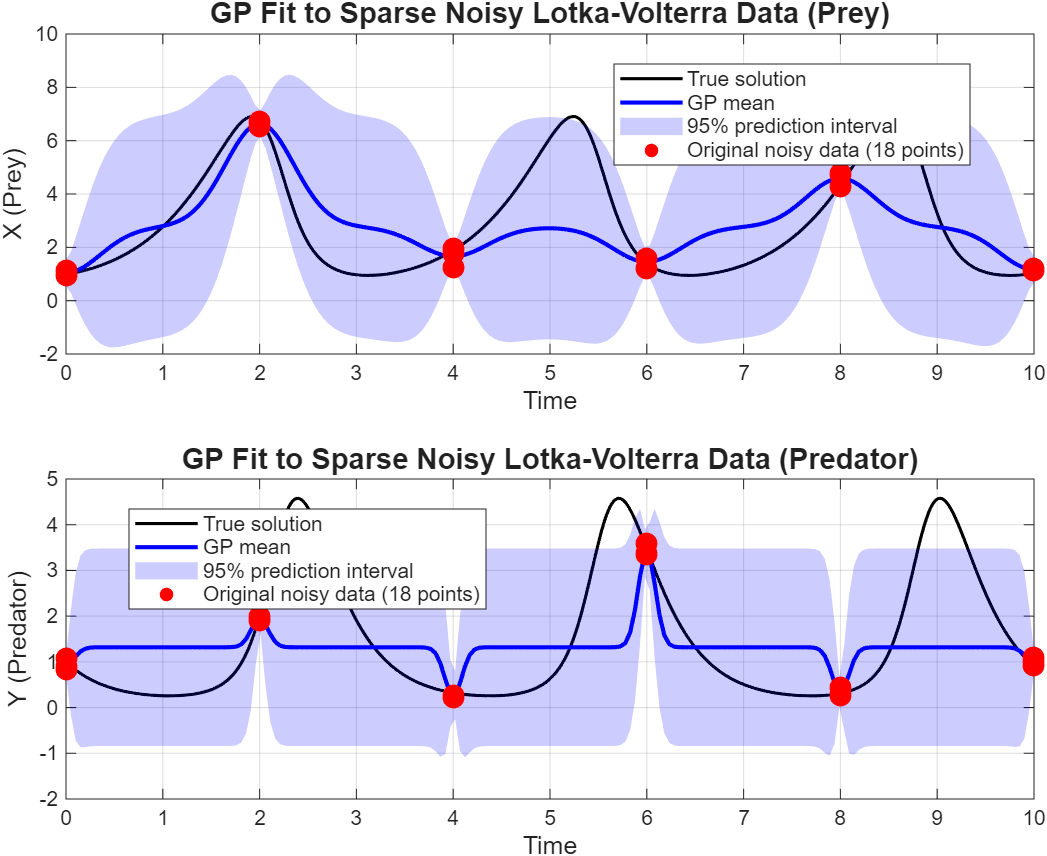
\includegraphics[width=0.8\textwidth]{figure1_gp_fit.png}
\caption{GP fit to sparse noisy Lotka-Volterra data showing mean predictions (blue), uncertainty bands (shaded), and original data points (red). The squared exponential kernel with constant basis provides smooth interpolation between sparse observations.}
\label{fig:gp_fit}
\end{figure}

\subsection{Analytical Derivative Computation}

A critical component of Path 2 is computing derivatives from the GP rather than using finite differences on noisy data. We implemented analytical derivative computation for the squared exponential kernel, which leverages the fact that the derivative of a GP is itself a GP. This provides smooth, denoised derivative estimates that are far superior to finite differences on sparse, noisy observations. The implementation includes a robust fallback mechanism: if the analytical derivatives are unreliable (detected by near-zero variance), the code automatically switches to finite differences computed on the GP mean predictions, which are still smoother than the raw data.

\begin{figure}[h]
\centering
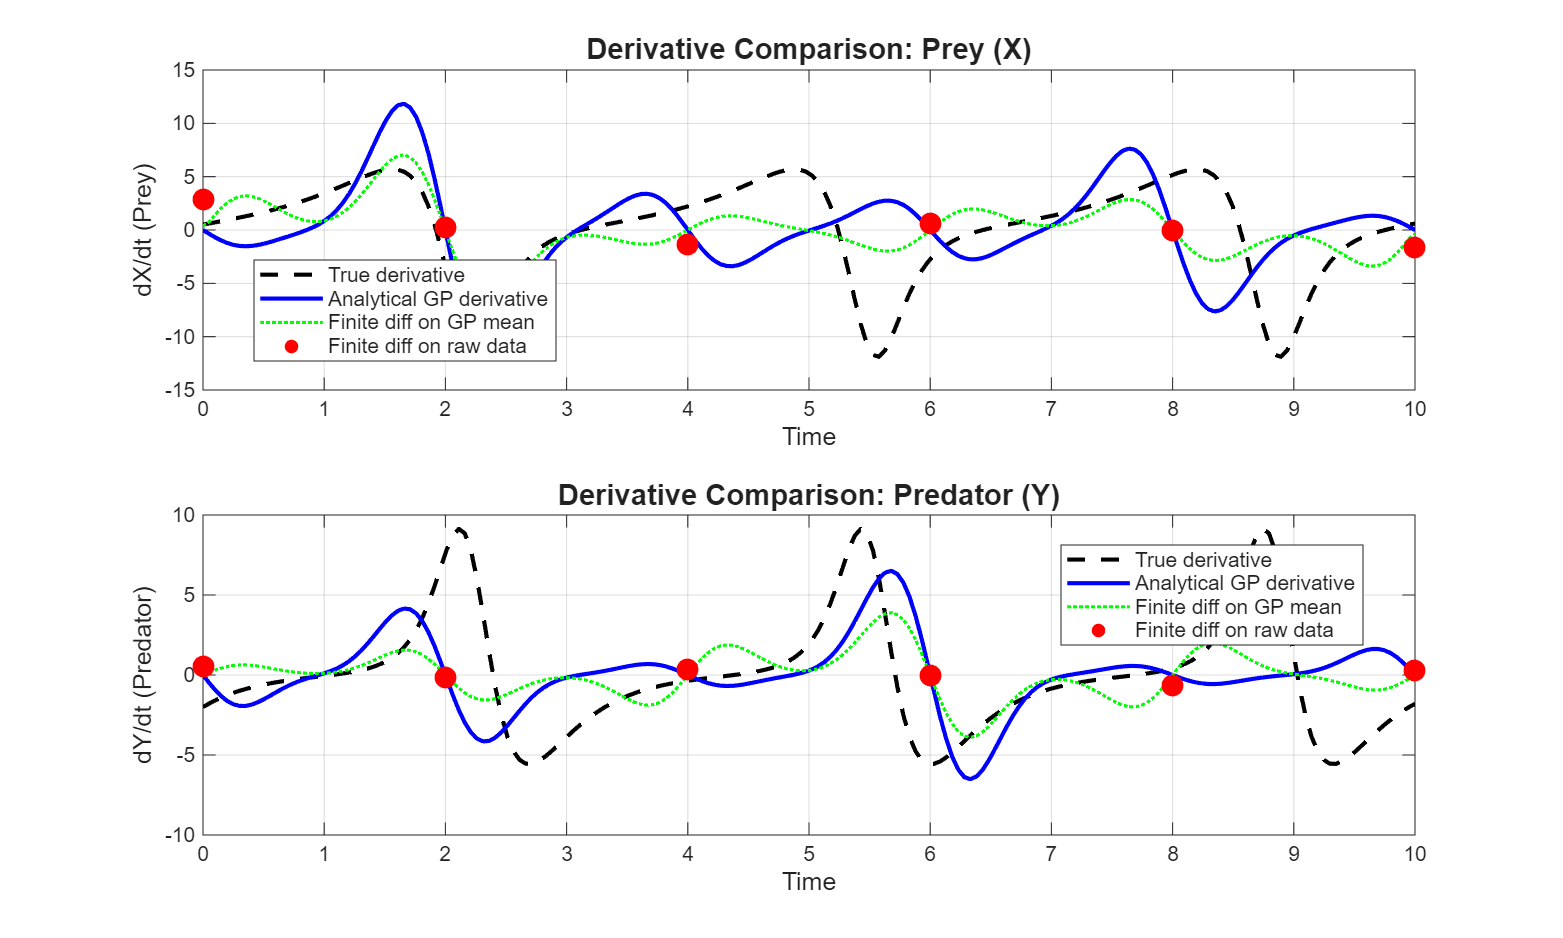
\includegraphics[width=0.8\textwidth]{figure2_derivatives.png}
\caption{Comparison of analytical GP derivatives (blue) versus finite differences on raw data (red) and true derivatives (black dashed). The GP derivatives provide smooth estimates that capture the underlying dynamics despite sparse, noisy observations.}
\label{fig:derivatives}
\end{figure}

\subsection{Posterior Sampling Strategy}

Rather than simply using the GP mean or adding independent noise, we implemented proper posterior sampling---drawing full curves from the GP posterior distribution. This respects the covariance structure of the GP and provides realistic variability. We combine the GP mean (at even-indexed time points) with GP samples (at odd-indexed time points), preserving the original data points at their exact locations. This strategy gives ESINDy a richer dataset (50 points instead of 6) while maintaining connection to the original observations.

\subsection{Kernel Selection Journey}

We explored multiple kernel options during development. The rational quadratic kernel initially seemed promising due to its flexibility, but it proved problematic---the GP optimization frequently converged to degenerate solutions with near-zero length scales, causing numerical instability in derivative computation. The squared exponential kernel, while simpler, proved more robust for sparse data scenarios and has well-established analytical derivative formulas. This choice aligns with the GP-ODE literature and provides the stability needed for reliable derivative computation.

\section{Current Status}

\subsection{What's Working}

The GP fitting pipeline is now functional and producing high-quality results:
\begin{itemize}
    \item Stable GP fits with squared exponential kernel and constant basis function
    \item Reliable analytical derivative computation
    \item Proper posterior sampling for data augmentation
    \item Robust fallback mechanisms for edge cases
    \item Path 1 (direct ESINDy) producing reasonable models with RMSE around 0.14
\end{itemize}

\begin{figure}[h]
\centering
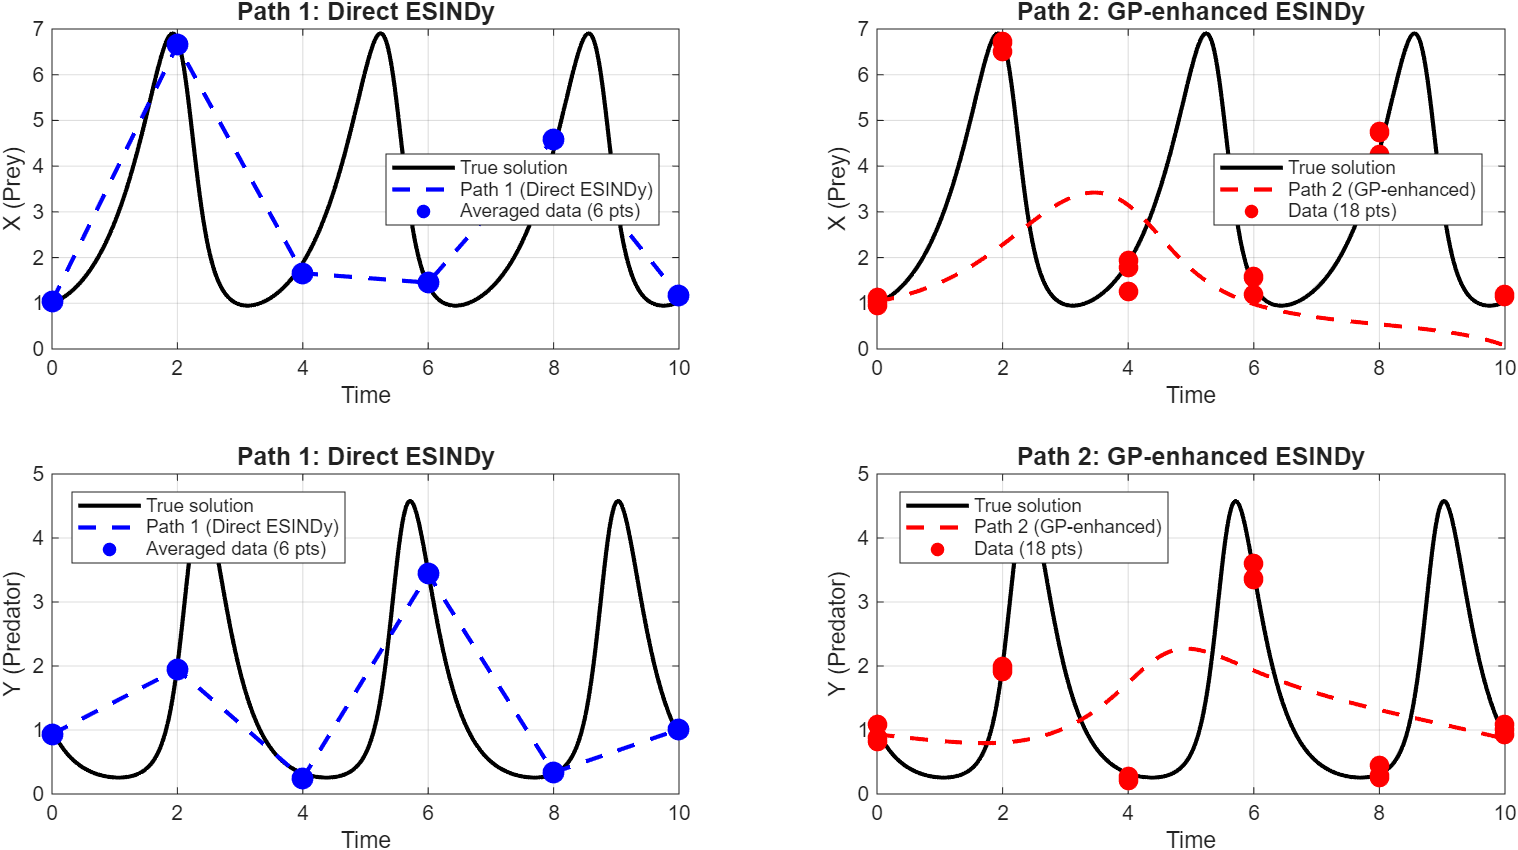
\includegraphics[width=0.8\textwidth]{figure3_model_comparison.png}
\caption{Model predictions comparison: true Lotka-Volterra solution (black), Path 1 predictions (blue), Path 2 predictions (red), and original sparse noisy data (red stars). Path 1 shows reasonable performance, while Path 2 requires further refinement.}
\label{fig:comparison}
\end{figure}

\subsection{What We're Still Working On}

Path 2 (GP-enhanced ESINDy) is currently experiencing model instability issues. While the GP components are working well, the final ESINDy models are producing high RMSE values and sometimes failing during numerical integration. This appears to be related to:

\begin{itemize}
    \item \textbf{Overfitting with expanded library:} The expanded function library (10 terms including cubic interactions) may be too complex for the available data, even after GP augmentation
    \item \textbf{Integration stability:} Some discovered models may be numerically unstable, requiring tighter tolerances or different integration methods
    \item \textbf{Regularization:} The sparsity threshold may need adjustment for the expanded library to prevent overfitting
    \item \textbf{Model selection:} We may need cross-validation or information criteria to select appropriate library terms rather than using all 10 functions
\end{itemize}

The GP infrastructure is solid, but the downstream ESINDy component needs refinement to fully realize the benefits of the augmented dataset.

\section{Key Takeaways}

This session successfully established a robust GP-enhanced pipeline for sparse data system identification. The squared exponential kernel with constant basis function provides stable, high-quality fits and reliable analytical derivatives. The posterior sampling approach gives principled data augmentation. However, the challenge of balancing model complexity (expanded library) with data availability remains, and this is the focus of ongoing work.

The foundation is in place---we have working GP fitting, derivative computation, and sampling. The next phase involves refining the ESINDy model selection and regularization to fully leverage the GP-augmented data.

\end{document}

